\documentclass[tikz,border=6pt]{standalone}
\usepackage[utf8]{inputenc}
\usepackage{amsmath}
\usepackage{xcolor}
\usetikzlibrary{arrows.meta,calc,angles,quotes}
\definecolor{azul}{HTML}{1E3A8A}
\definecolor{azul2}{HTML}{2563EB}
\definecolor{rojo}{HTML}{DC2626}
\definecolor{verde}{HTML}{16A34A}
\definecolor{gris}{HTML}{64748B}
\definecolor{naranja}{HTML}{F59E0B}
\begin{document}
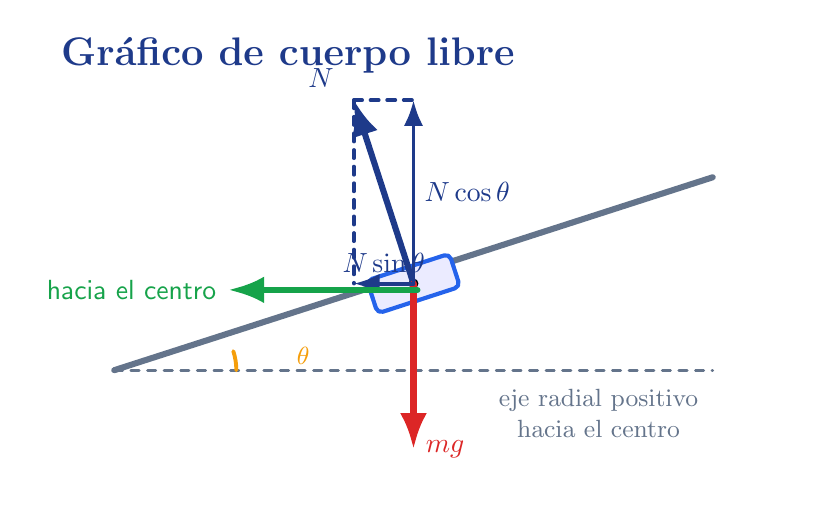
\begin{tikzpicture}[>=Latex, line cap=round, line join=round, font=\sffamily]
  % Fondo y marco lógico
  \fill[white] (-4.9,-2.8) rectangle (5.0,3.25);
  \node[azul, font=\bfseries\Large, anchor=west] at (-4.6,2.9) {Gráfico de cuerpo libre};

  % Parámetros geométricos
  \coordinate (O) at (0,0);            % partícula / centro del cuerpo
  \def\ang{18}                         % ángulo de peralte respecto horizontal
  \def\Nlen{2.45}
  \def\mglen{2.1}
  \def\comp{1.55}

  % Plano peraltado: sube hacia la derecha, centro hacia la izquierda
  \draw[gris, line width=2.2pt] (-3.8,-1.10) -- (3.8,1.35);
  \draw[gris, line width=1pt, dashed] (-3.8,-1.10) -- (3.8,-1.10);
  \draw[naranja, line width=1.4pt] (-2.25,-1.10) arc[start angle=0, end angle=18, radius=0.78];
  \node[naranja, font=\small] at (-1.40,-0.92) {$\theta$};

  % Bloque esquemático sobre la superficie
  \begin{scope}[rotate=\ang]
    \draw[azul2, line width=1.5pt, rounded corners=2pt, fill=blue!8] (-0.55,-0.22) rectangle (0.55,0.22);
  \end{scope}
  \fill[black] (O) circle (1.8pt);

  % Fuerzas reales
  \draw[->, azul, line width=2.2pt] (O) -- ++({90+\ang}:\Nlen) node[above left, xshift=-1mm] {$N$};
  \draw[->, rojo, line width=2.2pt] (O) -- ++(0,-\mglen) node[right] {$mg$};

  % Componentes de la normal: vertical y radial horizontal
  \coordinate (Ntip) at ($(O)+({90+\ang}:\Nlen)$);
  \coordinate (Vcomp) at ($(O)+(0,{\Nlen*cos(\ang)})$);
  \coordinate (Hcomp) at ($(O)+({-\Nlen*sin(\ang)},0)$);
  \draw[azul, dashed, line width=1.3pt] (Ntip) -- (Vcomp);
  \draw[azul, dashed, line width=1.3pt] (Ntip) -- (Hcomp);
  \draw[->, azul, line width=1.4pt] (O) -- (Vcomp) node[midway,right] {$N\cos\theta$};
  \draw[->, azul, line width=1.4pt] (O) -- (Hcomp) node[midway,above] {$N\sin\theta$};

  % Dirección hacia el centro
  \draw[->, verde, line width=2.2pt] (0.05,-0.08) -- (-2.35,-0.08) node[left] {hacia el centro};

  % Nota de ejes
  \node[gris, align=center, font=\small] at (2.35,-1.65) {eje radial positivo\\hacia el centro};
\end{tikzpicture}
\end{document}
